% Provenance (never printed): cycle 4 SVT, "La planete Terre, l'environnement
% et l'action humaine": the relief as a balance between uplift and erosion;
% landforms of the wind, the sea and dissolution; reading a landscape; see
% sources/book1/PROVENANCE.md. Book 1, grade 9, chapter 4.
% Vocabulary guard: owns uplift, dune, cliff, beach and spit (with longshore
% drift), karst (with cave and sinkhole). Landscape and landform are g1's;
% weathering, erosion, deposition, meander and delta are g5's; relief is
% g4's; plates and mountain building are g7's; U-shaped valley and moraine
% are g8's; limestone and the acid test are g6's; acids are the chemistry
% books' (recalled in prose). Contour lines are g9.5's (not used here).
% "Normal fault" and the destruction of mountains are Book 2's.
\chapter{Las formas del relieve}\label{ch:g9:landforms}

En la \omterm{def:g1:landscapes-around-us:water}{costa} sur de Inglaterra, los \omterm{def:g9:landforms:cliff}{acantilados} blancos de las Seven Sisters
caen a pico sobre el \omterm{def:g2:water-on-earth:ocean}{mar}. En un año normal pierden hasta un metro. En el
invierno de 2014, las \omterm{def:g5:natural-hazards:storm}{tormentas} se llevaron de los \omterm{def:g9:landforms:cliff}{acantilados} de Birling
Gap, en dos meses, tanto como suelen perder en siete años. La creta de
estos \omterm{def:g9:landforms:cliff}{acantilados} fue en otro tiempo \omterm{def:g3:stones-pebbles-sand:sand}{barro} del fondo de un \omterm{def:g2:water-on-earth:ocean}{mar}, formado por
las diminutas placas de las algas microscópicas que vivían en sus aguas.
Hoy se alza como una muralla de \omterm{def:g3:stones-pebbles-sand:rock}{roca} blanca que las olas hacen retroceder
un poco más cada año. ¿Por qué tiene el terreno las formas que tiene, y por
qué algunas cambian tan deprisa?
% ledger: nt:birling-2014, sdnp:birling, nasa:coccoliths

\begin{omfigure}
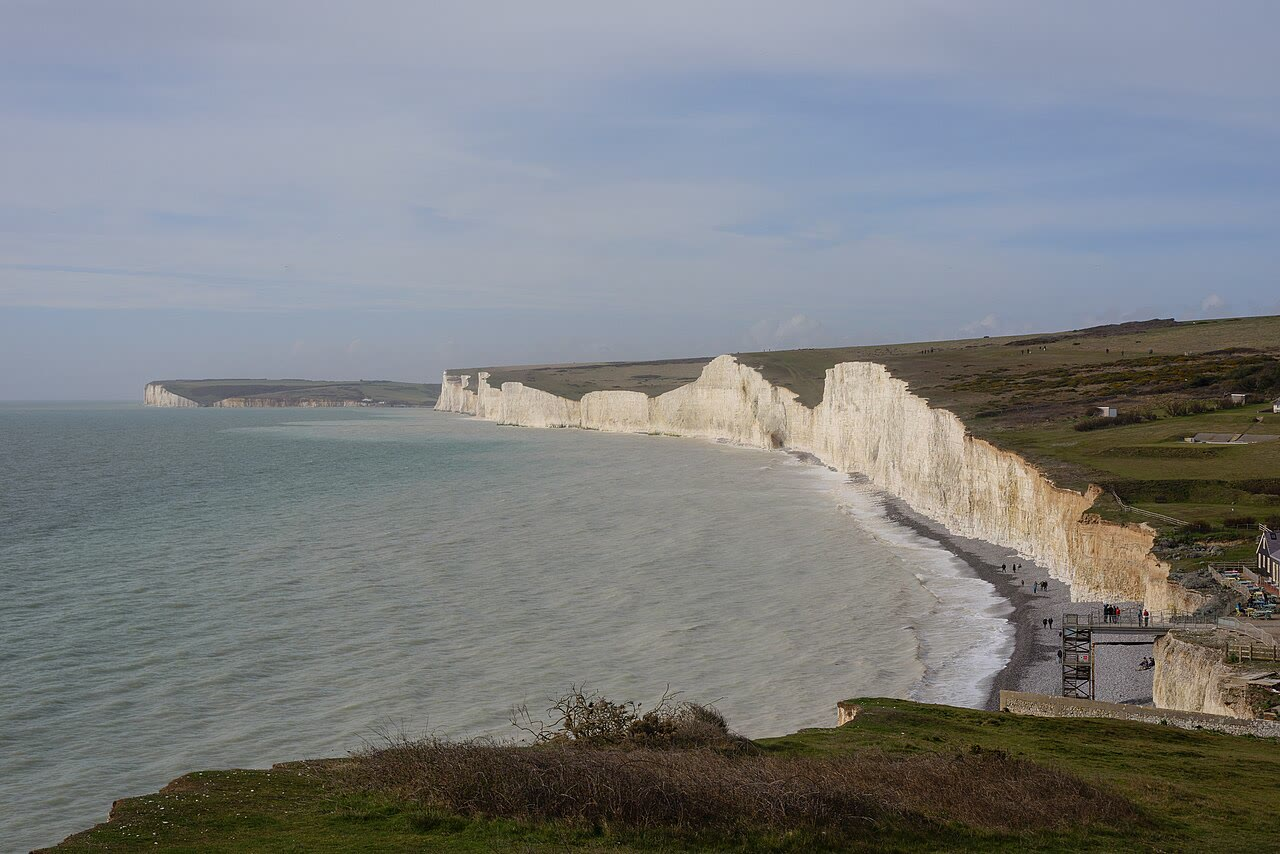
\includegraphics[width=\linewidth]{images/book1/g9-seven-sisters.jpg}

{\small Las Seven Sisters, \omterm{def:g9:landforms:cliff}{acantilados} de creta de la \omterm{def:g1:landscapes-around-us:water}{costa} de East Sussex
(Inglaterra), con las casas de Birling Gap en primer plano. El \omterm{def:g2:water-on-earth:ocean}{mar} hace
retroceder los \omterm{def:g9:landforms:cliff}{acantilados}, y los desprendimientos de \omterm{def:g3:stones-pebbles-sand:rock}{rocas} pueden
producirse en cualquier momento. A su pie se extiende una \omterm{def:g9:landforms:beach}{playa} de \omterm{def:g3:stones-pebbles-sand:pebble}{cantos}.
Fotografía de Arild Vågen, 2017 (CC BY-SA 4.0, vía Wikimedia Commons).}
% ledger: commons:seven-sisters, sdnp:birling
\label{fig:g9:landforms:seven-sisters}
\end{omfigure}

\begin{recall}
Una \emph{\omterm{def:g1:landscapes-around-us:landform}{forma del relieve}} es una de las formas del terreno: una \omterm{def:g1:landscapes-around-us:landform}{colina},
un \omterm{def:g1:landscapes-around-us:landform}{valle}, una \omterm{def:g1:landscapes-around-us:landform}{llanura}, un \omterm{def:g9:landforms:cliff}{acantilado} (\cref{ch:g1:landscapes-around-us}).
El \omterm{def:g4:world-physical-map:relief}{relieve} es la forma del terreno en altura
(\cref{ch:g4:world-physical-map}). La \omterm{def:g5:water-shapes-the-land:weathering}{meteorización} rompe la \omterm{def:g3:stones-pebbles-sand:rock}{roca}, la
\omterm{def:g5:water-shapes-the-land:erosion}{erosión} la desgasta y se la lleva, y la \omterm{def:g5:water-shapes-the-land:deposition}{sedimentación} la deposita en otro
lugar (\cref{ch:g5:water-shapes-the-land}). Las \omterm{def:g7:plate-tectonics:plate}{placas} levantan \omterm{def:g4:world-physical-map:range}{cordilleras}
donde chocan (\cref{ch:g7:plate-tectonics}); los \omterm{def:g8:ice-on-earth:glacier}{glaciares} excavan \omterm{def:g8:ice-on-earth:glacial-landforms}{valles
en U} (\cref{ch:g8:ice-on-earth}); la caliza hace efervescencia bajo una
gota de ácido diluido (\cref{ch:g6:rocks-and-minerals}). En química se
aprende que los ácidos atacan la caliza y desprenden dióxido de carbono.
\end{recall}

\section{El relieve: un equilibrio entre levantamiento y erosión}

Dos tipos de fuerzas modelan el \omterm{def:g4:world-physical-map:relief}{relieve}. Desde el interior, los
movimientos de las \omterm{def:g7:plate-tectonics:plate}{placas} elevan el terreno. Desde el exterior, el agua,
el hielo, el viento y el \omterm{def:g2:water-on-earth:ocean}{mar} lo desgastan.

\begin{definition}[Levantamiento]\label{def:g9:landforms:uplift}
El \emph{levantamiento}\index{levantamiento} es la lenta elevación de las
\omterm{def:g3:stones-pebbles-sand:rock}{rocas} y de la superficie del terreno de una región, causada por fuerzas
del interior de la Tierra, como la colisión de dos \omterm{def:g7:plate-tectonics:plate}{placas}.
\end{definition}

El \omterm{def:g9:landforms:uplift}{levantamiento} es lento a la escala de una vida, pero rápido a la escala
de la Tierra. La India chocó con Asia hace unos 50~millones de años, y la
meseta del Tíbet, detrás del Himalaya, ganó la mayor parte de su altura,
unos \qty{4600}{m}, en los últimos 10~millones de años. De media, eso son
$4600 \div 10^7 = 4.6 \times 10^{-4}$~m, o alrededor de \qty{0.5}{mm} al
año: menos que el grosor de una uña, pero mantenido durante millones de
años.
% ledger: usgs:himalaya (rate computed in figdata/grade-9/cliff_retreat.py, tibet_rate_mm_yr)

En cuanto el terreno se eleva, la \omterm{def:g5:water-shapes-the-land:erosion}{erosión} lo ataca. Cuanto más alto y más
empinado es el terreno, más deprisa se llevan la \omterm{def:g3:stones-pebbles-sand:rock}{roca} los \omterm{def:g1:landscapes-around-us:water}{ríos}, los
\omterm{def:g8:ice-on-earth:glacier}{glaciares} y los desprendimientos. La altura de una \omterm{def:g4:world-physical-map:range}{cordillera} en cada
momento es el resultado de una competición: lo que aporta el
\omterm{def:g9:landforms:uplift}{levantamiento}, menos lo que se lleva la \omterm{def:g5:water-shapes-the-land:erosion}{erosión}.

\begin{omfigure}
\begin{tikzpicture}[font=\footnotesize, >={Stealth[length=2mm]}]
  % panel 1: uplift faster than erosion
  \begin{scope}
    \fill[black!13] (0,0) -- (0.5,0) .. controls (1.1,1.0) and (1.5,2.0) .. (1.8,2.2)
      .. controls (2.1,2.0) and (2.5,1.0) .. (3.1,0) -- (3.6,0) -- (3.6,-0.5) -- (0,-0.5) -- cycle;
    \draw[black!60] (0,0) -- (0.5,0) .. controls (1.1,1.0) and (1.5,2.0) .. (1.8,2.2)
      .. controls (2.1,2.0) and (2.5,1.0) .. (3.1,0) -- (3.6,0);
    \draw[black!60, dashed] (0.7,0) .. controls (1.2,0.8) and (1.5,1.5) .. (1.8,1.6)
      .. controls (2.1,1.5) and (2.4,0.8) .. (2.9,0);
    \foreach \x in {1.2,1.8,2.4} \draw[->, omWarm, line width=1.4pt] (\x,-0.45) -- ++(0,1.0);
    \draw[->, omRiver, thick] (2.15,1.6) -- ++(0.35,-0.3);
    \node[align=center, anchor=north] at (1.8,-0.6) {levantamiento más rápido que\\la erosión: el relieve sube};
  \end{scope}
  % panel 2: uplift equals erosion
  \begin{scope}[xshift=4.4cm]
    \fill[black!13] (0,0) -- (0.5,0) .. controls (1.1,1.0) and (1.5,1.8) .. (1.8,1.9)
      .. controls (2.1,1.8) and (2.5,1.0) .. (3.1,0) -- (3.6,0) -- (3.6,-0.5) -- (0,-0.5) -- cycle;
    \draw[black!60] (0,0) -- (0.5,0) .. controls (1.1,1.0) and (1.5,1.8) .. (1.8,1.9)
      .. controls (2.1,1.8) and (2.5,1.0) .. (3.1,0) -- (3.6,0);
    \foreach \x in {1.2,1.8,2.4} \draw[->, omWarm, line width=1.4pt] (\x,-0.45) -- ++(0,0.6);
    \draw[->, omRiver, thick] (2.05,1.6) -- ++(0.55,-0.5);
    \draw[->, omRiver, thick] (1.55,1.6) -- ++(-0.55,-0.5);
    \node[align=center, anchor=north] at (1.8,-0.6) {levantamiento y erosión iguales:\\la altura no cambia};
  \end{scope}
  % panel 3: no more uplift
  \begin{scope}[xshift=8.8cm]
    \fill[black!13] (0,0) -- (0.4,0) .. controls (1.1,0.5) and (1.5,0.95) .. (1.8,1.0)
      .. controls (2.1,0.95) and (2.5,0.5) .. (3.2,0) -- (3.6,0) -- (3.6,-0.5) -- (0,-0.5) -- cycle;
    \draw[black!60] (0,0) -- (0.4,0) .. controls (1.1,0.5) and (1.5,0.95) .. (1.8,1.0)
      .. controls (2.1,0.95) and (2.5,0.5) .. (3.2,0) -- (3.6,0);
    \draw[black!60, dashed] (0.5,0) .. controls (1.1,1.0) and (1.5,1.8) .. (1.8,1.9)
      .. controls (2.1,1.8) and (2.5,1.0) .. (3.1,0);
    \draw[->, omRiver, thick] (2.05,0.95) -- ++(0.55,-0.5);
    \draw[->, omRiver, thick] (1.55,0.95) -- ++(-0.55,-0.5);
    \node[align=center, anchor=north] at (1.8,-0.6) {sin levantamiento: la erosión\\rebaja el relieve};
  \end{scope}
  % key
  \draw[->, omWarm, line width=1.4pt] (13.2,1.2) -- ++(0,0.6) node[right, black] {levantamiento};
  \draw[->, omRiver, thick] (13.2,0.7) -- ++(0.35,-0.3) node[right, black] {erosión};
  \draw[black!60, dashed] (13.1,-0.1) -- ++(0.5,0) node[right, black] {perfil anterior};
\end{tikzpicture}

{\small El \omterm{def:g4:world-physical-map:relief}{relieve} como un equilibrio (un esquema, no a escala). El
\omterm{def:g9:landforms:uplift}{levantamiento} eleva las \omterm{def:g3:stones-pebbles-sand:rock}{rocas}; la \omterm{def:g5:water-shapes-the-land:erosion}{erosión} se las lleva hacia los \omterm{def:g1:landscapes-around-us:landform}{valles} y
el \omterm{def:g2:water-on-earth:ocean}{mar}. Una \omterm{def:g4:world-physical-map:range}{cordillera} sigue creciendo mientras gana el \omterm{def:g9:landforms:uplift}{levantamiento};
cuando las \omterm{def:g7:plate-tectonics:plate}{placas} dejan de empujar, la \omterm{def:g5:water-shapes-the-land:erosion}{erosión} la desgasta lentamente
hasta dejarla en \omterm{def:g1:landscapes-around-us:landform}{colinas}.}
\label{fig:g9:landforms:balance}
\end{omfigure}

Los \omterm{def:g1:landscapes-around-us:water}{ríos} (\cref{ch:g5:water-shapes-the-land}) y los \omterm{def:g8:ice-on-earth:glacier}{glaciares}
(\cref{ch:g8:ice-on-earth}) son los grandes escultores de las \omterm{def:g1:landscapes-around-us:landform}{montañas}. El
resto de este capítulo sigue a otros tres agentes, que crean \omterm{def:g1:landscapes-around-us:landform}{formas del
relieve} propias: el viento, el \omterm{def:g2:water-on-earth:ocean}{mar} y el agua que disuelve la \omterm{def:g3:stones-pebbles-sand:rock}{roca}.

\section{Las formas creadas por el viento: las dunas}

Donde hay pocas plantas, abundante \omterm{def:g3:stones-pebbles-sand:sand}{arena} suelta y un viento fuerte, el
viento puede levantar la \omterm{def:g3:stones-pebbles-sand:sand}{arena} y amontonarla en \omterm{def:g1:landscapes-around-us:landform}{colinas}: en los \omterm{def:g5:weather-and-climate:desert}{desiertos},
y detrás de las \omterm{def:g9:landforms:beach}{playas} de \omterm{def:g3:stones-pebbles-sand:sand}{arena}.
% ledger: nps:aeolian

\begin{definition}[Duna]\label{def:g9:landforms:dune}
Una \emph{duna}\index{duna} es un montículo o una cresta de \omterm{def:g3:stones-pebbles-sand:sand}{arena} suelta
amontonada por el viento. Su ladera de cara al viento es larga y suave; su
lado opuesto, la \emph{cara de avalancha}\index{cara de avalancha}, es
corto y empinado.
\end{definition}
% ledger: nps:aeolian, nmt:barchan

Una \omterm{def:g9:landforms:dune}{duna} se desplaza. El viento hace rodar y rebotar los granos ladera
arriba por la pendiente suave; en la cresta se amontonan hasta que el
montón se vuelve demasiado empinado, y una pequeña avalancha de \omterm{def:g3:stones-pebbles-sand:sand}{arena} se
desliza por la \omterm{def:g9:landforms:dune}{cara de avalancha}. Grano a grano, la \omterm{def:g3:stones-pebbles-sand:sand}{arena} se toma del lado
de barlovento y se deposita en el lado opuesto, y la \omterm{def:g9:landforms:dune}{duna} entera avanza en
el sentido del viento sin levantarse nunca. Las \omterm{def:g9:landforms:dune}{dunas} rara vez están
solas: cubren campos enteros.
% ledger: nmt:barchan, nps:aeolian

Donde el viento sopla siempre desde la misma dirección y la \omterm{def:g3:stones-pebbles-sand:sand}{arena} no es
demasiado abundante, las \omterm{def:g9:landforms:dune}{dunas} toman forma de media luna, un
\emph{barján}: su frente redondeado mira al viento y sus dos cuernos
apuntan en el sentido del viento. Los cuernos contienen menos \omterm{def:g3:stones-pebbles-sand:sand}{arena} que el
centro, así que avanzan más deprisa y se adelantan a la \omterm{def:g9:landforms:dune}{duna}.
% ledger: nmt:barchan

\begin{omfigure}
\begin{tikzpicture}[font=\footnotesize, >={Stealth[length=2mm]}]
  % plan view
  \fill[yellow!25!orange!20] (3.4,1.3) .. controls (1.0,1.3) and (0.2,0.6) .. (0.2,0)
     .. controls (0.2,-0.6) and (1.0,-1.3) .. (3.4,-1.3)
     .. controls (2.4,-0.9) and (1.8,-0.5) .. (1.8,0)
     .. controls (1.8,0.5) and (2.4,0.9) .. (3.4,1.3) -- cycle;
  \fill[orange!45] (3.4,1.3) .. controls (2.4,0.9) and (1.8,0.5) .. (1.8,0)
     .. controls (1.8,-0.5) and (2.4,-0.9) .. (3.4,-1.3)
     .. controls (2.1,-0.8) and (1.45,-0.45) .. (1.45,0)
     .. controls (1.45,0.45) and (2.1,0.8) .. (3.4,1.3) -- cycle;
  \draw[black!60] (3.4,1.3) .. controls (1.0,1.3) and (0.2,0.6) .. (0.2,0)
     .. controls (0.2,-0.6) and (1.0,-1.3) .. (3.4,-1.3)
     .. controls (2.4,-0.9) and (1.8,-0.5) .. (1.8,0)
     .. controls (1.8,0.5) and (2.4,0.9) .. (3.4,1.3);
  \draw[black, thick] (3.4,1.3) .. controls (2.1,0.8) and (1.45,0.45) .. (1.45,0)
     .. controls (1.45,-0.45) and (2.1,-0.8) .. (3.4,-1.3);
  \foreach \y in {-0.8,0,0.8} \draw[->, omRiver, thick] (-1.3,\y) -- ++(1.1,0);
  \node[above] at (-0.75,0.85) {viento};
  \node[anchor=west] at (3.5,1.35) {cuerno};
  \node[anchor=west] at (3.5,-1.35) {cuerno};
  \draw[black!70] (1.75,0.25) -- (2.9,0.35) node[anchor=west, align=left, black] {cara de avalancha\\(empinada)};
  \draw[black!70] (0.75,-0.2) -- (0.6,-1.6) node[anchor=north, align=center, black] {ladera de barlovento\\(suave)};
  \draw[black!70] (1.47,-0.3) -- (2.4,-1.75) node[anchor=north, black] {cresta};
  \node[anchor=south, font=\footnotesize\bfseries] at (1.4,1.6) {vista desde arriba};
  % profile
  \begin{scope}[xshift=7.2cm, yshift=-0.8cm]
    \draw[black!60] (-0.4,0) -- (5.6,0);
    \fill[yellow!25!orange!20] (0,0) -- (3.0,1.2) -- (3.6,0) -- cycle;
    \draw[black!70] (0,0) -- (3.0,1.2) -- (3.6,0);
    \fill[orange!45] (3.0,1.2) -- (3.6,0) -- (3.3,0) -- cycle;
    \draw[black!50, dashed] (0.8,0) -- (3.8,1.2) -- (4.4,0);
    \draw[->, black!70] (0.5,0.35) .. controls (0.75,0.65) .. (1.0,0.45);
    \draw[->, black!70] (1.0,0.55) .. controls (1.25,0.85) .. (1.5,0.65);
    \draw[->, black!70] (1.5,0.75) .. controls (1.75,1.05) .. (2.0,0.85);
    \draw[->, black!70] (2.0,0.95) .. controls (2.25,1.25) .. (2.5,1.05);
    \draw[->, thick, black!80] (3.15,1.05) -- (3.45,0.35);
    \foreach \y in {1.6,2.1} \draw[->, omRiver, thick] (-0.8,\y) -- ++(1.1,0);
    \node[above] at (-0.25,2.1) {viento};
    \draw[->, thick] (4.5,0.6) -- ++(0.7,0) node[right, align=left] {la duna\\avanza};
    \node[align=center, anchor=north] at (1.2,-0.1) {los granos suben rebotando\\por la pendiente suave};
    \node[align=center, anchor=north west] at (2.9,-0.1) {y se deslizan por\\la cara de avalancha};
    \node[anchor=south, font=\footnotesize\bfseries] at (2.2,2.3) {vista de perfil};
  \end{scope}
\end{tikzpicture}

{\small Una \omterm{def:g9:landforms:dune}{duna} en media luna, o barján (un esquema). Vista desde arriba,
sus cuernos apuntan en el sentido del viento. Vista de perfil, los granos
suben por la suave ladera de barlovento y se deslizan por la empinada \omterm{def:g9:landforms:dune}{cara
de avalancha}: la \omterm{def:g9:landforms:dune}{duna} avanza en el sentido del viento (contorno
discontinuo: la \omterm{def:g9:landforms:dune}{duna} un poco más tarde).}
% ledger: nmt:barchan, nps:aeolian
\label{fig:g9:landforms:barchan}
\end{omfigure}

¿A qué velocidad? En el campo de \omterm{def:g9:landforms:dune}{dunas} de yeso de White Sands, en Nuevo
México, las \omterm{def:g9:landforms:dune}{dunas} pequeñas que se forman en su borde de barlovento, de
unos pocos metros de altura, avanzan hasta \qty{6}{m} al año; un poco más
lejos, cuando han crecido hasta 6 a \qty{10}{m} de altura, avanzan unos
\qty{3}{m} al año. Cuanta más \omterm{def:g3:stones-pebbles-sand:sand}{arena} contiene una \omterm{def:g9:landforms:dune}{duna}, más despacio va.
Los barjanes empujados por vientos fuertes pueden recorrer más de
\qty{100}{m} en un año, lo suficiente para enterrar una carretera o un
campo.
% ledger: nps:whsa-migration, nmt:barchan

\begin{omfigure}
\begin{minipage}[c]{0.5\linewidth}\centering
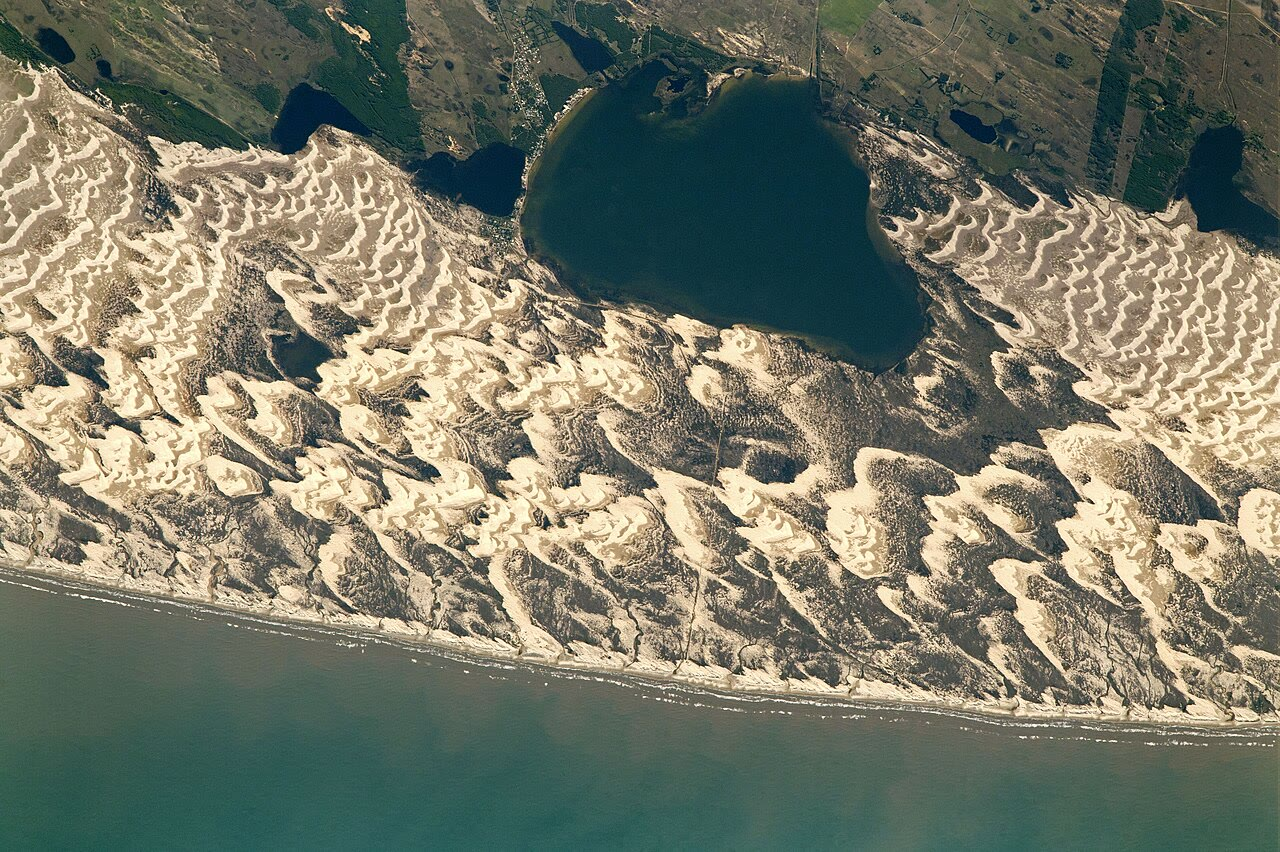
\includegraphics[width=\linewidth]{images/book1/g9-barchans.jpg}
\end{minipage}\hfill
\begin{minipage}[c]{0.46\linewidth}\raggedright
{\small \omterm{def:g9:landforms:dune}{Dunas} en media luna en la \omterm{def:g1:landscapes-around-us:water}{costa} atlántica del sur de Brasil,
fotografiadas por un astronauta desde la Estación Espacial Internacional
en 2017. El \omterm{def:g1:landscapes-around-us:water}{lago} oscuro, la Lagoa dos \omterm{def:g3:stones-pebbles-sand:sand}{Barros}, mide unos \qty{4.5}{km} de
largo. La \omterm{def:g3:stones-pebbles-sand:sand}{arena} procede de la \omterm{def:g9:landforms:beach}{playa}, en la parte inferior de la
fotografía. NASA (dominio público, vía Wikimedia Commons).}
\end{minipage}
% ledger: commons:iss-barchans
\label{fig:g9:landforms:barchans-photo}
\end{omfigure}

En una \omterm{def:g1:landscapes-around-us:water}{costa}, una hilera de \omterm{def:g9:landforms:dune}{dunas} detrás de la \omterm{def:g9:landforms:beach}{playa} protege el terreno de
detrás de las olas de las \omterm{def:g5:natural-hazards:storm}{tormentas}. Las plantas que crecen en las \omterm{def:g9:landforms:dune}{dunas}
sujetan la \omterm{def:g3:stones-pebbles-sand:sand}{arena} con sus raíces: donde se pisotean o se arrancan, el
viento vuelve a llevarse la \omterm{def:g3:stones-pebbles-sand:sand}{arena}.
% ledger: nps:aeolian

\section{Las formas creadas por el mar}

\subsection{Los acantilados}

\begin{definition}[Acantilado]\label{def:g9:landforms:cliff}
Un \emph{acantilado}\index{acantilado} es una pared de \omterm{def:g3:stones-pebbles-sand:rock}{roca} empinada o
vertical. En una \omterm{def:g1:landscapes-around-us:water}{costa}, el acantilado lo labran las olas, que atacan su
pie y lo hacen retroceder tierra adentro.
\end{definition}

Las olas lanzan agua, \omterm{def:g3:stones-pebbles-sand:sand}{arena} y \omterm{def:g3:stones-pebbles-sand:pebble}{cantos} contra el pie del \omterm{def:g9:landforms:cliff}{acantilado}. Poco a
poco excavan un hueco en su base, una \emph{muesca}, entre los niveles de
la marea baja y de la marea alta. La \omterm{def:g3:stones-pebbles-sand:rock}{roca} de encima queda en voladizo; la
\omterm{def:g4:clouds-rain-snow:precipitation}{lluvia} y la helada la debilitan aún más. Un día, el voladizo se derrumba.
Las olas rompen los bloques caídos y se los llevan, y el ataque vuelve a
empezar en una pared nueva, un poco más hacia el interior. Detrás de sí, el
\omterm{def:g9:landforms:cliff}{acantilado} deja una superficie de \omterm{def:g3:stones-pebbles-sand:rock}{roca} plana, la \emph{plataforma de
abrasión}\index{plataforma de abrasion@plataforma de abrasión}, que aparece
con la marea baja.
% ledger: nt:birling-2014, sdnp:birling

Las \omterm{def:g3:stones-pebbles-sand:rock}{rocas} blandas son las que retroceden más deprisa. En Birling Gap, los
\omterm{def:g9:landforms:cliff}{acantilados} de creta pierden hasta alrededor de un metro al año; pero el
retroceso se produce a saltos, un desprendimiento tras otro, y un invierno
tormentoso puede llevarse de una vez varios años de retroceso. En 1999, el
antiguo faro de Belle Tout, construido en 1832 en lo alto de los
\omterm{def:g9:landforms:cliff}{acantilados} cercanos, se desplazó entero \qty{17}{m} hacia atrás desde el
borde, porque el \omterm{def:g9:landforms:cliff}{acantilado} se estaba acercando demasiado.
% ledger: sdnp:birling, nt:birling-2014

\begin{omfigure}
\begin{tikzpicture}[font=\footnotesize, >={Stealth[length=2mm]}]
  % panel 1: the notch
  \begin{scope}
    \fill[omSea!45] (0,-0.1) rectangle (1.8,0.75);
    \fill[omSea!45] (1.8,0.35) -- (2.25,0.55) -- (1.8,0.95) -- cycle;
    \fill[black!8] (1.6,-0.1) -- (1.8,0.25) -- (1.8,0.35) -- (2.25,0.55) -- (1.8,0.95) -- (1.8,2.4) -- (3.6,2.4) -- (3.6,-0.6) -- (0,-0.6) -- (0,-0.1) -- cycle;
    \draw[black!70] (0,-0.1) -- (1.6,-0.1) -- (1.8,0.25) -- (1.8,0.35) -- (2.25,0.55) -- (1.8,0.95) -- (1.8,2.4) -- (3.6,2.4);
    \foreach \y in {0.8,1.3,1.8} \draw[black!25] (1.8,\y) -- (3.6,\y);
    \fill[green!35!black!50] (1.8,2.4) rectangle (3.6,2.5);
    \draw[->, omSea!80!black, thick] (0.4,0.6) -- (1.6,0.6);
    \node[anchor=south, align=center] at (0.9,0.8) {olas};
    \draw[black!70] (2.15,0.55) -- (2.9,1.0) node[anchor=west, fill=white, inner sep=1pt] {muesca};
    \node[anchor=north, align=center] at (1.8,-0.7) {1. las olas excavan\\una muesca};
    \node[anchor=south, font=\footnotesize] at (2.7,2.5) {creta};
  \end{scope}
  % panel 2: collapse
  \begin{scope}[xshift=4.6cm]
    \fill[omSea!45] (0,-0.1) rectangle (2.2,0.75);
    \fill[black!8] (2.0,-0.1) -- (2.2,0.25) -- (2.25,2.4) -- (3.6,2.4) -- (3.6,-0.6) -- (0,-0.6) -- (0,-0.1) -- cycle;
    \draw[black!70] (0,-0.1) -- (2.0,-0.1) -- (2.2,0.25) -- (2.25,2.4) -- (3.6,2.4);
    \draw[black!50, dashed] (1.8,0.95) -- (1.8,2.4) -- (2.25,2.4);
    \foreach \y in {0.8,1.3,1.8} \draw[black!25] (2.25,\y) -- (3.6,\y);
    \fill[green!35!black!50] (2.25,2.4) rectangle (3.6,2.5);
    \foreach \x/\y/\s in {1.25/0.05/0.28, 1.6/0.1/0.22, 1.95/0.3/0.3, 1.45/0.35/0.18}
      \fill[black!20, draw=black!60] (\x,\y) rectangle ++(\s,\s*0.8);
    \node[anchor=north, align=center] at (1.8,-0.7) {2. el voladizo\\se derrumba};
  \end{scope}
  % panel 3: retreat and platform
  \begin{scope}[xshift=9.2cm]
    \fill[omSea!45] (0,0.2) rectangle (2.8,0.75);
    \fill[black!8] (0,0.0) -- (2.6,0.2) -- (2.8,0.3) -- (2.85,2.4) -- (4.0,2.4) -- (4.0,-0.6) -- (0,-0.6) -- cycle;
    \draw[black!70] (0,0.0) -- (2.6,0.2) -- (2.8,0.3) -- (2.85,2.4) -- (4.0,2.4);
    \foreach \y in {0.8,1.3,1.8} \draw[black!25] (2.85,\y) -- (4.0,\y);
    \fill[green!35!black!50] (2.85,2.4) rectangle (4.0,2.5);
    \draw[black!50, dashed] (1.4,0.12) -- (1.4,2.4);
    \draw[black!50, dashed] (2.1,0.16) -- (2.1,2.4);
    \draw[<-, thick] (2.8,1.6) -- (1.5,1.6);
    \node[anchor=south, align=center] at (1.4,2.45) {antiguas paredes};
    \node[anchor=north, align=center] at (2.0,-0.7) {3. una plataforma de abrasión,\\descubierta con la marea baja};
  \end{scope}
\end{tikzpicture}

{\small Cómo retrocede un \omterm{def:g9:landforms:cliff}{acantilado} marino (un esquema, no a escala).
(1) Las olas excavan una muesca al pie del \omterm{def:g9:landforms:cliff}{acantilado}. (2) La \omterm{def:g3:stones-pebbles-sand:rock}{roca} en
voladizo se derrumba; las olas rompen los bloques y se los llevan. (3) El
ciclo se repite: el \omterm{def:g9:landforms:cliff}{acantilado} avanza tierra adentro y deja delante una
plataforma de \omterm{def:g3:stones-pebbles-sand:rock}{roca} plana.}
% ledger: nt:birling-2014, sdnp:birling
\label{fig:g9:landforms:cliff-retreat}
\end{omfigure}

\begin{safety}
El borde de un \omterm{def:g9:landforms:cliff}{acantilado} puede ceder en cualquier momento, y de la pared
caen \omterm{def:g3:stones-pebbles-sand:rock}{rocas} sin aviso. Los \omterm{def:g9:landforms:cliff}{acantilados} se observan desde una distancia
segura, bien lejos del borde arriba y bien lejos del pie en la \omterm{def:g9:landforms:beach}{playa}, y se
abandona una \omterm{def:g9:landforms:beach}{playa} al pie de \omterm{def:g9:landforms:cliff}{acantilados} antes de que suba la marea.
\end{safety}
% ledger: nt:birling-2014, sdnp:birling

\subsection{Playas y flechas litorales}

La \omterm{def:g3:stones-pebbles-sand:sand}{arena} y los \omterm{def:g3:stones-pebbles-sand:pebble}{cantos} arrancados a los \omterm{def:g9:landforms:cliff}{acantilados}, y los que bajan los
\omterm{def:g1:landscapes-around-us:water}{ríos}, no se quedan donde caen: las olas los clasifican y los desplazan a
lo largo de la \omterm{def:g1:landscapes-around-us:water}{costa}.

\begin{definition}[Playa, deriva litoral y flecha litoral]\label{def:g9:landforms:beach}
Una \emph{playa}\index{playa} es una franja de \omterm{def:g3:stones-pebbles-sand:sand}{arena} o de \omterm{def:g3:stones-pebbles-sand:pebble}{cantos}
amontonados por las olas a lo largo de la orilla. Cuando las olas llegan a
la orilla en ángulo, cada ola empuja los granos playa arriba con ese
ángulo, y el agua vuelve a bajar en línea recta por la pendiente: los
granos avanzan en zigzag a lo largo de la \omterm{def:g1:landscapes-around-us:water}{costa}. Este desplazamiento de
\omterm{def:g3:stones-pebbles-sand:sand}{arena} y \omterm{def:g3:stones-pebbles-sand:pebble}{cantos} a lo largo de la orilla es la \emph{deriva
litoral}\index{deriva litoral}. Una
\emph{flecha litoral}\index{flecha litoral} es una cresta larga y
estrecha de \omterm{def:g3:stones-pebbles-sand:sand}{arena} o de \omterm{def:g3:stones-pebbles-sand:pebble}{cantos} construida por la deriva litoral, unida a tierra por un extremo y que se adentra en el
\omterm{def:g2:water-on-earth:ocean}{mar} donde la \omterm{def:g1:landscapes-around-us:water}{costa} gira.
\end{definition}
% ledger: noaa:longshore

Donde la \omterm{def:g1:landscapes-around-us:water}{costa} se curva, a la entrada de una bahía o en la \omterm{def:g5:water-shapes-the-land:source-mouth}{desembocadura} de
un \omterm{def:g1:landscapes-around-us:water}{río}, la deriva sigue en la misma dirección y deposita su carga en el
agua más tranquila: la \omterm{def:g9:landforms:beach}{playa} crece \omterm{def:g2:water-on-earth:ocean}{mar} adentro en forma de flecha. Su
extremo suele curvarse hacia dentro, doblado por olas que llegan de otras
direcciones. Detrás de la flecha, al abrigo de las olas, se deposita el
\omterm{def:g3:stones-pebbles-sand:sand}{barro} y crecen marismas.
% ledger: noaa:longshore

\begin{omfigure}
\begin{tikzpicture}[font=\footnotesize, >={Stealth[length=2mm]}]
  % sea
  \fill[omSea!40] (0,0) rectangle (11,2.3);
  % land with a bay
  \fill[green!25!black!20] (0,2.3) -- (6,2.3) .. controls (6.3,3.0) and (7.0,3.5) .. (8.0,3.5)
     .. controls (9.0,3.5) and (9.3,2.8) .. (9.5,2.3) -- (11,2.3) -- (11,4.6) -- (0,4.6) -- cycle;
  % calm water of the bay
  \fill[omSea!20] (6,2.3) .. controls (6.3,3.0) and (7.0,3.5) .. (8.0,3.5)
     .. controls (9.0,3.5) and (9.3,2.8) .. (9.5,2.3) -- cycle;
  % salt marsh
  \fill[green!50!black!35] (6.15,2.55) .. controls (6.6,3.1) and (7.3,3.2) .. (7.9,3.0)
     .. controls (7.6,2.7) and (7.0,2.6) .. (6.15,2.55) -- cycle;
  \node[anchor=west, font=\scriptsize] at (6.5,3.85) {marisma};
  \draw[black!60] (6.9,3.75) -- (7.0,2.95);
  % river
  \draw[omRiver, line width=1.2pt] (8.6,4.6) .. controls (8.5,4.0) and (8.3,3.7) .. (8.3,3.48);
  \node[anchor=west, font=\scriptsize] at (8.65,4.25) {río};
  % beach
  \fill[yellow!40!orange!35] (0,1.85) rectangle (6,2.3);
  % spit
  \fill[yellow!40!orange!35] (5.9,1.85) .. controls (7.0,1.95) and (7.8,2.0) .. (8.35,2.1)
     .. controls (8.6,2.2) and (8.6,2.5) .. (8.4,2.65) -- (8.25,2.55)
     .. controls (8.35,2.45) and (8.3,2.35) .. (8.15,2.32)
     .. controls (7.5,2.28) and (6.8,2.3) .. (6.0,2.3) -- cycle;
  \draw[black!60] (0,2.3) -- (6,2.3) .. controls (6.3,3.0) and (7.0,3.5) .. (8.0,3.5)
     .. controls (9.0,3.5) and (9.3,2.8) .. (9.5,2.3) -- (11,2.3);
  % waves arriving at an angle
  \foreach \x in {0.9,2.0,3.1,4.2} \draw[omSea!70!black, line width=0.5pt] (\x,1.15) -- ++(-35:1.1);
  \draw[->, omSea!70!black, thick] (0.6,0.3) -- ++(55:1.2) node[pos=0.15, left, black] {olas};
  % zigzag of a pebble
  \draw[->, black, thick] (1.0,1.9) -- (1.35,2.2) -- (1.35,1.9) -- (1.7,2.2) -- (1.7,1.9)
     -- (2.05,2.2) -- (2.05,1.9) -- (2.4,2.2) -- (2.4,1.9);
  \node[anchor=south, align=center, font=\scriptsize] at (1.7,2.45) {suben en ángulo,\\vuelven a bajar\\en línea recta};
  % drift arrow
  \draw[->, line width=1.6pt, omWarm] (3.0,1.55) -- (5.6,1.55) node[midway, below, black] {deriva litoral};
  % spit label
  \draw[black!70] (7.4,2.05) -- (7.6,1.2) node[anchor=north, align=center, black] {la flecha crece\\a través de la bahía};
  \draw[->, thick, omWarm] (8.6,1.95) -- ++(0.6,0);
  % compass
  \draw[->] (10.4,0.3) -- ++(0,0.6) node[above] {N};
\end{tikzpicture}

{\small La \omterm{def:g9:landforms:beach}{deriva litoral} y una \omterm{def:g9:landforms:beach}{flecha litoral}, vistas desde arriba (un
esquema). Las olas llegan del suroeste; cada una empuja la \omterm{def:g3:stones-pebbles-sand:sand}{arena} y los
\omterm{def:g3:stones-pebbles-sand:pebble}{cantos} \omterm{def:g9:landforms:beach}{playa} arriba en ángulo, y el agua vuelve a bajar en línea recta: los
granos avanzan en zigzag hacia el este. Donde la \omterm{def:g1:landscapes-around-us:water}{costa} gira para formar una
bahía, la deriva continúa y construye una flecha, detrás de la cual crece
una marisma. El \omterm{def:g1:landscapes-around-us:water}{río} mantiene un canal abierto en el extremo de la flecha.}
% ledger: noaa:longshore
\label{fig:g9:landforms:spit}
\end{omfigure}

\begin{omfigure}
\begin{minipage}[c]{0.5\linewidth}\centering
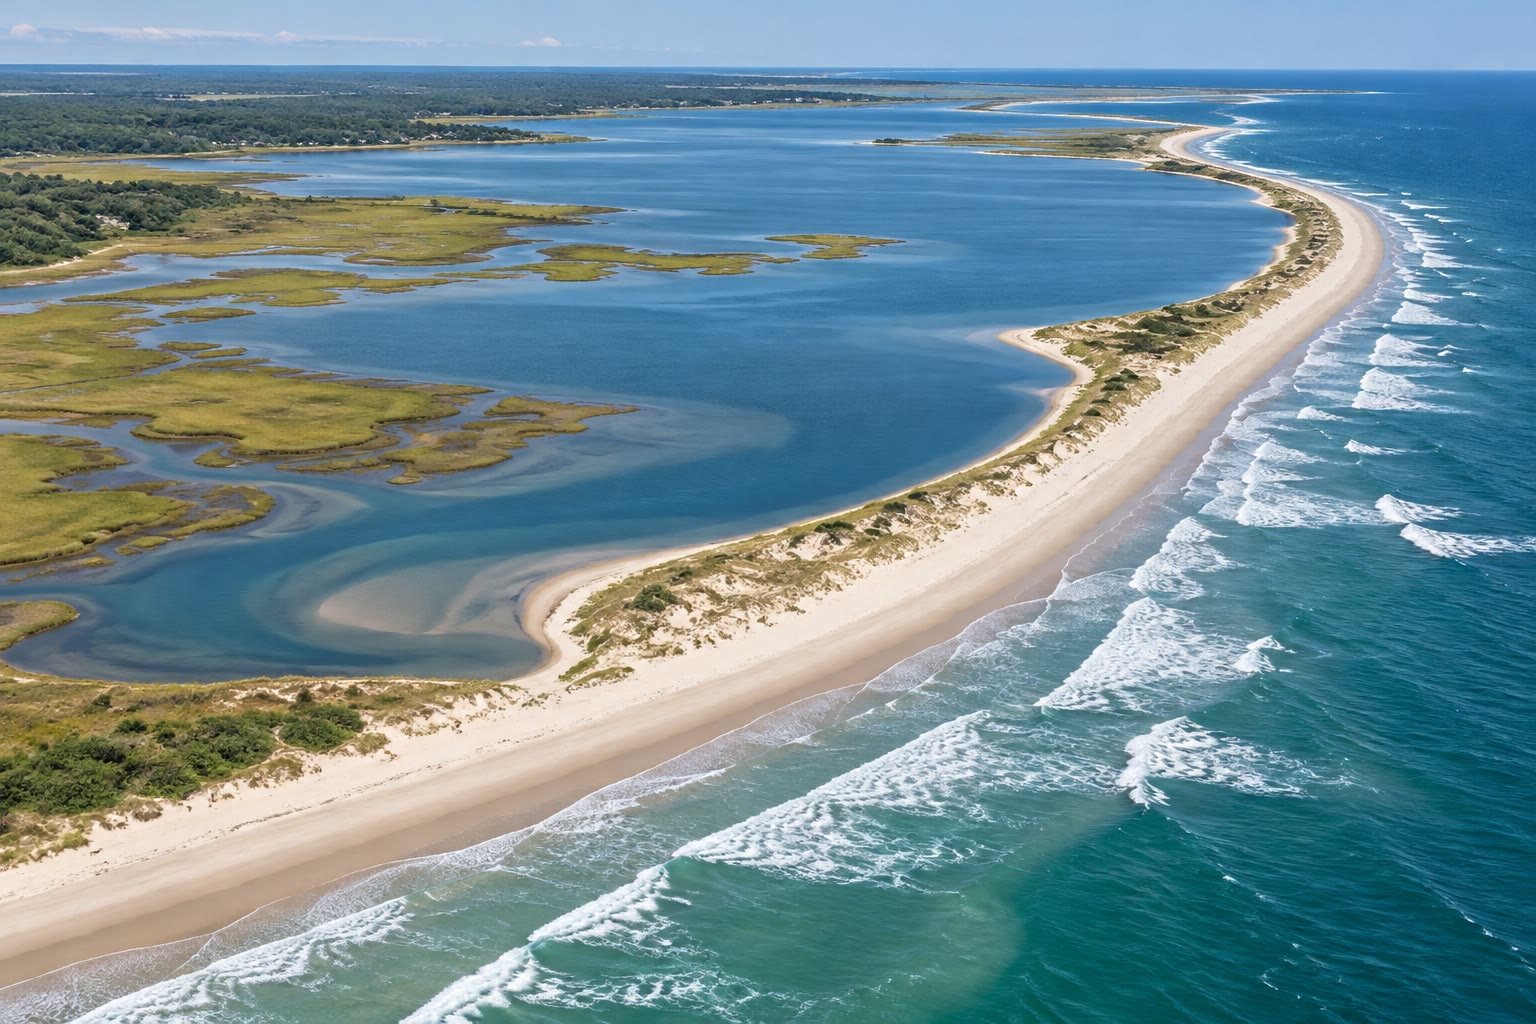
\includegraphics[width=\linewidth]{images/book1/ai/g9-spit-aerial.jpg}
\end{minipage}\hfill
\begin{minipage}[c]{0.46\linewidth}\raggedright
{\small Una flecha de \omterm{def:g3:stones-pebbles-sand:sand}{arena} a través de la entrada de una bahía, vista
desde una avioneta a baja altura (una ilustración, no un lugar real). Las
olas rompen en su \omterm{def:g9:landforms:beach}{playa} del lado del \omterm{def:g2:water-on-earth:ocean}{mar}; detrás quedan aguas tranquilas y
marismas.}
\end{minipage}
\label{fig:g9:landforms:spit-ai}
\end{omfigure}

\section{Las formas creadas por la disolución: el karst}

El agua de \omterm{def:g4:clouds-rain-snow:precipitation}{lluvia} no es agua pura. Al caer a través del aire y al
infiltrarse después en el suelo, absorbe dióxido de carbono, que la vuelve
ligeramente ácida. Este ácido débil hace despacio lo que la gota de ácido
diluido hace deprisa con un trozo de caliza: disuelve la \omterm{def:g3:stones-pebbles-sand:rock}{roca}. La caliza
está llena de grietas, a lo largo de sus capas y a través de ellas. El
agua se filtra por ellas y las ensancha, milímetro a milímetro, a lo largo
de miles de años.
% ledger: usgs:sinkholes, nps:karst

\begin{definition}[Karst, cueva y dolina]\label{def:g9:landforms:karst}
Un \emph{karst}\index{karst} es un \omterm{def:g1:landscapes-around-us:landscape}{paisaje} modelado por el agua que
disuelve una \omterm{def:g3:stones-pebbles-sand:rock}{roca} soluble, casi siempre caliza. Los \omterm{def:g1:landscapes-around-us:water}{ríos} tienden allí a
desaparecer bajo tierra y a volver a salir en forma de \omterm{def:g6:water-underground:spring}{manantiales}. Una
\emph{cueva}\index{cueva} es un espacio subterráneo natural lo bastante
grande para que entre una persona, disuelto a lo largo de las grietas de
la \omterm{def:g3:stones-pebbles-sand:rock}{roca}. Una \emph{dolina}\index{dolina} es una depresión o un agujero en
la superficie del terreno, formado donde la \omterm{def:g3:stones-pebbles-sand:rock}{roca} de debajo se disuelve o
donde se hunde el techo de una cueva.
\end{definition}
% ledger: nps:karst, usgs:sinkholes

\begin{omfigure}
\begin{tikzpicture}[x=0.9cm, y=0.9cm, font=\footnotesize, >={Stealth[length=2mm]}]
  \pic (B) at (0,0) {blockdiagram={10}{4}{4}};
  % top face: grassland
  \fill[green!25!black!18] (B-ftl) -- (B-ftr) -- (B-btr) -- (B-btl) -- cycle;
  % right face
  \fill[omLithLime!70] (B-fbr) -- (B-bbr) -- (B-btr) -- (B-ftr) -- cycle;
  % front face: limestone layers
  \fill[omLithLime] (B-fbl) rectangle (B-ftr);
  \foreach \y in {0.8,1.6,2.4,3.2} \draw[black!35] (0,\y) -- (10,\y);
  \foreach \x/\y in {1.2/0.8, 3.1/1.6, 4.6/0, 6.8/2.4, 8.3/0.8, 2.2/2.4, 9.1/2.4, 5.6/3.2}
    \draw[black!35] (\x,\y) -- ++(0,0.8);
  % soil
  \fill[brown!45] (0,3.8) rectangle (10,4);
  % sinkhole on the top face and in the front face
  \fill[green!25!black!35] (3.0,4.45) ellipse (0.7 and 0.22);
  \fill[white] (2.3,4) -- (3.7,4) -- (3.25,3.45) -- (2.75,3.45) -- cycle;
  \fill[green!25!black!30] (2.3,4) -- (3.7,4) -- (3.25,3.45) -- (2.75,3.45) -- cycle;
  \draw[black!60] (2.3,4) -- (2.75,3.45) -- (3.25,3.45) -- (3.7,4);
  % shaft from sinkhole to cave
  \fill[white] (2.85,3.45) -- (3.15,3.45) -- (3.35,2.0) -- (3.05,2.0) -- cycle;
  \draw[black!60] (2.85,3.45) -- (3.05,2.0) (3.15,3.45) -- (3.35,2.0);
  % cave
  \fill[white] (2.6,2.1) .. controls (3.5,2.35) and (5.5,2.3) .. (6.6,1.9)
     .. controls (7.4,1.6) and (7.6,1.2) .. (7.2,1.0)
     .. controls (6.0,0.85) and (4.0,1.0) .. (3.0,1.2)
     .. controls (2.3,1.35) and (2.1,1.9) .. (2.6,2.1) -- cycle;
  \draw[black!70] (2.6,2.1) .. controls (3.5,2.35) and (5.5,2.3) .. (6.6,1.9)
     .. controls (7.4,1.6) and (7.6,1.2) .. (7.2,1.0)
     .. controls (6.0,0.85) and (4.0,1.0) .. (3.0,1.2)
     .. controls (2.3,1.35) and (2.1,1.9) .. (2.6,2.1);
  % underground stream at the cave floor
  \fill[omRiver!60] (3.0,1.2) .. controls (4.0,1.0) and (6.0,0.85) .. (7.2,1.0) -- (7.1,1.12)
     .. controls (6.0,1.0) and (4.0,1.12) .. (3.1,1.3) -- cycle;
  % stalactites and stalagmites
  \foreach \x/\l in {4.2/0.35, 4.5/0.22, 4.9/0.4, 5.3/0.25, 5.8/0.3}
    \fill[black!45] (\x-0.07,2.22) -- (\x+0.06,2.22) -- (\x,2.22-\l) -- cycle;
  \foreach \x/\l in {4.9/0.3, 5.8/0.25}
    \fill[black!45] (\x-0.12,0.95) -- (\x+0.12,0.95) -- (\x,0.95+\l) -- cycle;
  % disappearing stream on the top face
  \draw[omRiver, line width=1.2pt] (7.4,4.85) .. controls (6.9,4.5) and (6.4,4.4) .. (6.0,4.25);
  \fill[black!70] (6.0,4.25) circle (0.07);
  \draw[omRiver, dashed, thick] (6.0,4.0) -- (6.4,2.1);
  % spring on the right face
  \draw[omRiver, line width=1.2pt, ->] (10.2,1.2) .. controls (10.8,1.1) and (11.2,0.7) .. (11.6,0.5);
  % rain with carbon dioxide
  \foreach \x in {0.6,1.2,1.8} \draw[->, omRiver] (\x,5.6) -- ++(-0.15,-0.7);
  \draw[->, omRiver, dashed] (1.0,3.9) -- (1.2,1.7);
  % outline
  \draw[black!70] (B-fbl) rectangle (B-ftr);
  \draw[black!70] (B-ftl) -- (B-btl) -- (B-btr) -- (B-ftr) (B-btr) -- (B-bbr) -- (B-fbr);
  % labels
  \node[anchor=south, align=center] at (1.2,5.6) {la lluvia absorbe dióxido\\de carbono: ligeramente ácida};
  \node[anchor=east, align=right] at (-0.1,1.6) {el agua ensancha\\las grietas};
  \draw[black!70] (-0.05,1.6) -- (1.1,2.0);
  \node[anchor=south] at (3.0,5.2) {dolina};
  \draw[black!70] (3.0,5.2) -- (3.0,4.55);
  \node[anchor=south, align=center] at (7.6,5.3) {un arroyo desaparece\\bajo tierra};
  \draw[black!70] (7.0,5.3) -- (6.1,4.35);
  \node[anchor=north, align=center] at (5.0,-0.1) {una cueva: las estalactitas cuelgan del techo,\\las estalagmitas se elevan desde el suelo};
  \draw[black!70] (5.0,-0.1) -- (5.0,1.4);
  \node[anchor=west, align=left] at (11.6,0.6) {manantial};
  \node[anchor=west] at (11.9,3.4) {caliza};
\end{tikzpicture}

{\small Un \omterm{def:g1:landscapes-around-us:landscape}{paisaje} kárstico (un esquema, no a escala). El agua
ligeramente ácida se filtra por las grietas de la caliza y las ensancha;
las corrientes subterráneas excavan \omterm{def:g9:landforms:karst}{cuevas}; el techo de una \omterm{def:g9:landforms:karst}{cueva} cede y
abre una \omterm{def:g9:landforms:karst}{dolina}; un arroyo desaparece por un agujero y vuelve a salir más
abajo en forma de \omterm{def:g6:water-underground:spring}{manantial}.}
% ledger: nps:karst, usgs:sinkholes, nps:speleothems
\label{fig:g9:landforms:karst}
\end{omfigure}

En una \omterm{def:g9:landforms:karst}{cueva}, la disolución puede funcionar al revés. Una gota de agua que
se filtra desde el techo lleva caliza disuelta. Cuando se encuentra con el
aire de la \omterm{def:g9:landforms:karst}{cueva}, desprende parte de su dióxido de carbono, y una fina
película de calcita sale del agua alrededor de la gota. Gota a gota, un
tubo hueco crece desde el techo y después se engrosa hasta convertirse en
una \emph{estalactita}\index{estalactita}, que cuelga como un carámbano.
Donde caen las gotas, el resto de la calcita construye una
\emph{estalagmita}\index{estalagmita} que se eleva desde el suelo. Cuando
las dos se juntan, forman una columna.
% ledger: nps:speleothems

\begin{omfigure}
\begin{minipage}[c]{0.5\linewidth}\centering
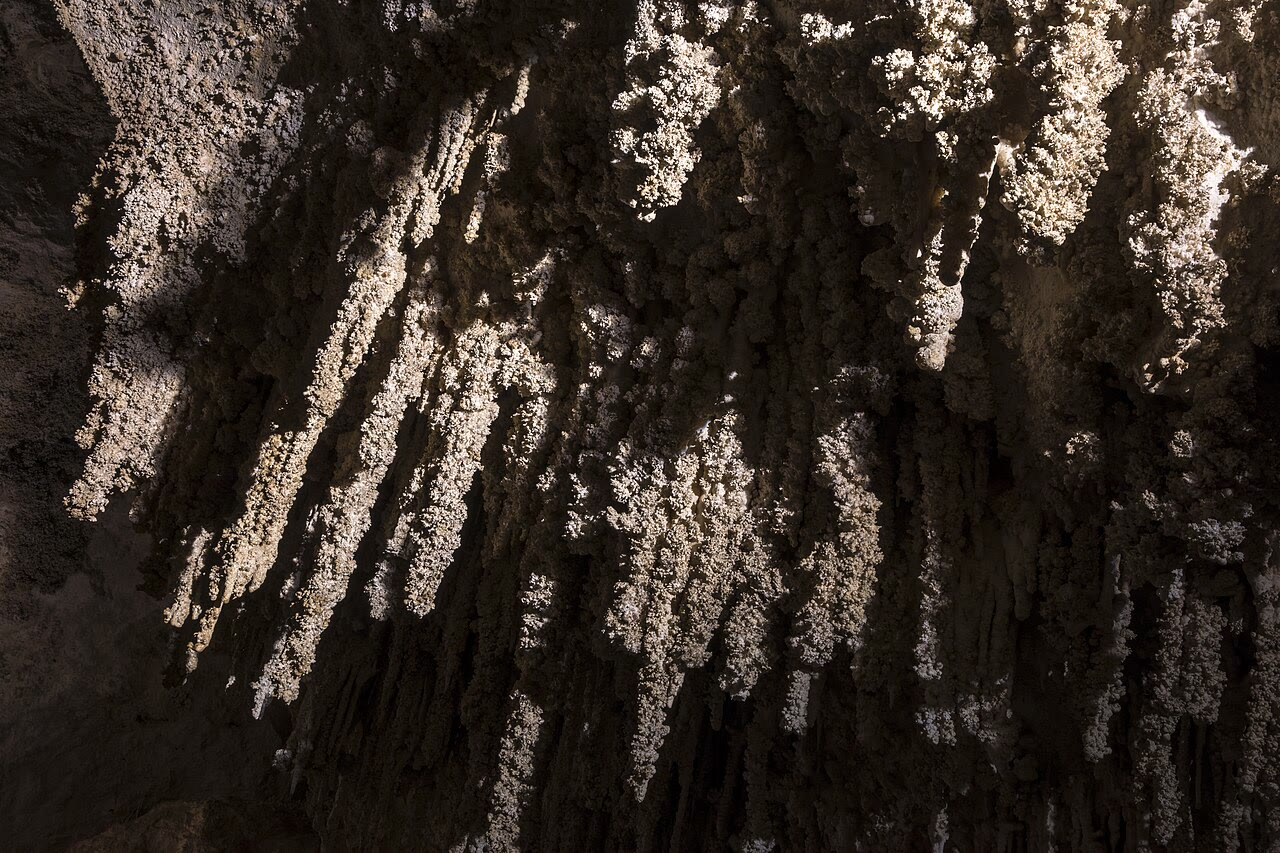
\includegraphics[width=\linewidth]{images/book1/g9-stalactites.jpg}
\end{minipage}\hfill
\begin{minipage}[c]{0.46\linewidth}\raggedright
{\small Estalactitas que cuelgan bajo un gran bloque de \omterm{def:g3:stones-pebbles-sand:rock}{roca} en la \omterm{def:g9:landforms:karst}{cueva} de
Carlsbad (Carlsbad Cavern), en Nuevo México, una \omterm{def:g9:landforms:karst}{cueva} disuelta en la
caliza. Cada una creció gota a gota a partir del agua que se filtraba por
la \omterm{def:g3:stones-pebbles-sand:rock}{roca} de encima. National Park Service, 2018 (dominio público, vía
Wikimedia Commons).}
\end{minipage}
% ledger: commons:carlsbad-stalactites, nps:speleothems
\label{fig:g9:landforms:stalactites}
\end{omfigure}

Las regiones kársticas guardan mucha agua bajo tierra, pero esta circula
deprisa por las grietas abiertas y apenas se filtra: cualquier cosa que se
derrame en el suelo puede llegar enseguida a un \omterm{def:g6:water-underground:spring}{manantial}. Y donde la \omterm{def:g3:stones-pebbles-sand:rock}{roca}
de debajo se ha disuelto, el terreno puede hundirse o desplomarse: donde
vive gente, una \omterm{def:g9:landforms:karst}{dolina} que se abre de repente puede tragarse carreteras y
casas.
% ledger: nps:karst, usgs:sinkholes

\section{Leer un paisaje}

Cada \omterm{def:g1:landscapes-around-us:landform}{forma del relieve} es una pista. Su forma indica qué agente la creó;
el agente indica qué proceso actuó, \omterm{def:g5:water-shapes-the-land:erosion}{erosión} o \omterm{def:g5:water-shapes-the-land:deposition}{sedimentación}; y el proceso
dice a menudo algo sobre la \omterm{def:g3:stones-pebbles-sand:rock}{roca} o el material suelto que hay debajo.

\begin{method}[Leer una forma del relieve]
\begin{enumerate}
  \item \textbf{Forma.} Describe la \omterm{def:g1:landscapes-around-us:landform}{forma del relieve}: una cresta, una
        depresión, una pared empinada, una superficie plana; su tamaño;
        hacia dónde apunta.
  \item \textbf{Agente y proceso.} Decide qué agente la creó (un \omterm{def:g1:landscapes-around-us:water}{río}, el
        hielo, el viento, el \omterm{def:g2:water-on-earth:ocean}{mar}, el agua que disuelve) y si se excavó
        (\omterm{def:g5:water-shapes-the-land:erosion}{erosión}) o se construyó (\omterm{def:g5:water-shapes-the-land:deposition}{sedimentación}).
  \item \textbf{Material.} Di de qué está hecha, o qué \omterm{def:g3:stones-pebbles-sand:rock}{roca} es probable que
        haya debajo: \omterm{def:g3:stones-pebbles-sand:sand}{arena} suelta, \omterm{def:g3:stones-pebbles-sand:pebble}{cantos}, caliza, \omterm{def:g3:stones-pebbles-sand:rock}{roca} dura o blanda.
\end{enumerate}
\end{method}

\begin{center}
{\small
\begin{tabular}{|>{\raggedright\arraybackslash}p{4.6cm}|>{\raggedright\arraybackslash}p{2.6cm}|>{\raggedright\arraybackslash}p{2.2cm}|>{\raggedright\arraybackslash}p{2.6cm}|}
\hline
forma & agente & proceso & material \\
\hline
\omterm{def:g1:landscapes-around-us:landform}{colinas} de \omterm{def:g3:stones-pebbles-sand:sand}{arena} en media luna & viento & \omterm{def:g5:water-shapes-the-land:deposition}{sedimentación} & \omterm{def:g3:stones-pebbles-sand:sand}{arena} suelta \\
una pared de \omterm{def:g3:stones-pebbles-sand:rock}{roca} vertical sobre una superficie de \omterm{def:g3:stones-pebbles-sand:rock}{roca} plana & \omterm{def:g2:water-on-earth:ocean}{mar} & \omterm{def:g5:water-shapes-the-land:erosion}{erosión} & \omterm{def:g3:stones-pebbles-sand:rock}{roca} (la \omterm{def:g3:stones-pebbles-sand:rock}{roca} blanda retrocede deprisa) \\
una cresta estrecha de \omterm{def:g3:stones-pebbles-sand:sand}{arena} a través de una bahía & \omterm{def:g2:water-on-earth:ocean}{mar} (\omterm{def:g9:landforms:beach}{deriva litoral}) & \omterm{def:g5:water-shapes-the-land:deposition}{sedimentación} & \omterm{def:g3:stones-pebbles-sand:sand}{arena} o \omterm{def:g3:stones-pebbles-sand:pebble}{cantos} \\
depresiones en los campos, arroyos que desaparecen & agua que disuelve & disolución & caliza \\
un \omterm{def:g8:ice-on-earth:glacial-landforms}{valle en U} & hielo & \omterm{def:g5:water-shapes-the-land:erosion}{erosión} & cualquier \omterm{def:g3:stones-pebbles-sand:rock}{roca} \\
un abanico de \omterm{def:g3:stones-pebbles-sand:sand}{barro} en la \omterm{def:g5:water-shapes-the-land:source-mouth}{desembocadura} de un \omterm{def:g1:landscapes-around-us:water}{río} & \omterm{def:g1:landscapes-around-us:water}{río} & \omterm{def:g5:water-shapes-the-land:deposition}{sedimentación} & \omterm{def:g3:stones-pebbles-sand:sand}{barro} y \omterm{def:g3:stones-pebbles-sand:sand}{arena} \\
\hline
\end{tabular}}
\end{center}

\begin{example}[Un paseo por una meseta]
En una alta meseta cubierta de hierba no hay ni un solo arroyo, aunque
llueve a menudo. Los campos están salpicados de depresiones redondas de
unos pocos metros de diámetro, y en el \omterm{def:g1:landscapes-around-us:landform}{valle} de abajo un potente \omterm{def:g6:water-underground:spring}{manantial}
brota al pie de una pared de \omterm{def:g3:stones-pebbles-sand:rock}{roca}. \emph{Forma}: depresiones, ningún arroyo
en la superficie, un \omterm{def:g6:water-underground:spring}{manantial} más abajo. \emph{Agente y proceso}: el agua
que disuelve la \omterm{def:g3:stones-pebbles-sand:rock}{roca} y circula bajo tierra. \emph{Material}: lo más
probable es que la meseta sea de caliza, y que las depresiones sean
\omterm{def:g9:landforms:karst}{dolinas}. Una gota de ácido diluido sobre un trozo suelto de la \omterm{def:g3:stones-pebbles-sand:rock}{roca},
puesta por el profesor, haría efervescencia.
\end{example}
% ledger: nps:karst, usgs:sinkholes

\section{Ejercicios}

\begin{exercise}[$\star$]\label{exo:g9:landforms:1}
¿Qué agente creó cada \omterm{def:g1:landscapes-around-us:landform}{forma del relieve}: el viento, el \omterm{def:g2:water-on-earth:ocean}{mar}, un \omterm{def:g1:landscapes-around-us:water}{río}, el
hielo o el agua que disuelve la \omterm{def:g3:stones-pebbles-sand:rock}{roca}? (a) Una \omterm{def:g1:landscapes-around-us:landform}{colina} de \omterm{def:g3:stones-pebbles-sand:sand}{arena} en media luna
en un \omterm{def:g5:weather-and-climate:desert}{desierto}. (b) Una \omterm{def:g9:landforms:karst}{cueva} llena de estalactitas. (c) Una larga cresta
de \omterm{def:g3:stones-pebbles-sand:pebble}{cantos} a través de la entrada de una bahía. (d) Un \omterm{def:g8:ice-on-earth:glacial-landforms}{valle en U} con una
\omterm{def:g8:ice-on-earth:glacial-landforms}{morrena} en su extremo. (e) Una pared vertical de creta con una superficie
de \omterm{def:g3:stones-pebbles-sand:rock}{roca} plana a su pie. (f) Un \omterm{def:g5:water-shapes-the-land:delta}{delta}.
\end{exercise}

\begin{exercise}[$\star$]\label{exo:g9:landforms:2}
Da la palabra que corresponde a cada descripción. (a) La lenta elevación de
las \omterm{def:g3:stones-pebbles-sand:rock}{rocas} y del terreno de una región. (b) El lado empinado de una \omterm{def:g9:landforms:dune}{duna},
opuesto al viento. (c) Un agujero en el terreno formado donde la \omterm{def:g3:stones-pebbles-sand:rock}{roca} de
debajo se ha disuelto o se ha hundido el techo de una \omterm{def:g9:landforms:karst}{cueva}. (d) El
desplazamiento de \omterm{def:g3:stones-pebbles-sand:sand}{arena} y \omterm{def:g3:stones-pebbles-sand:pebble}{cantos} a lo largo de la orilla. (e) Un \omterm{def:g1:landscapes-around-us:landscape}{paisaje}
modelado por el agua que disuelve la caliza.
\end{exercise}

\begin{exercise}[$\star$]\label{exo:g9:landforms:3}
¿Verdadero o falso? Corrige las frases falsas. (a) Los cuernos de una \omterm{def:g9:landforms:dune}{duna}
en media luna apuntan hacia el viento. (b) La ladera de una \omterm{def:g9:landforms:dune}{duna} que mira
al viento es suave. (c) Una \omterm{def:g9:landforms:dune}{duna} se desplaza porque el viento la levanta
entera de una vez. (d) Las \omterm{def:g9:landforms:dune}{dunas} se forman con más facilidad donde crecen
pocas plantas.
\end{exercise}

\begin{exercise}[$\star$]\label{exo:g9:landforms:4}
Ordena estas etapas del retroceso de un \omterm{def:g9:landforms:cliff}{acantilado} marino. (a) Las olas
rompen los bloques caídos y se los llevan. (b) Las olas excavan una muesca
al pie del \omterm{def:g9:landforms:cliff}{acantilado}. (c) La pared del \omterm{def:g9:landforms:cliff}{acantilado} está ahora más hacia el
interior, y la plataforma plana de delante es un poco más ancha. (d) La
\omterm{def:g3:stones-pebbles-sand:rock}{roca} situada encima de la muesca queda en voladizo. (e) El voladizo se
derrumba.
\end{exercise}

\begin{exercise}[$\star\star$]\label{exo:g9:landforms:5}
% ledger: nps:whsa-migration (6 and 3 m a year)
Vistas desde un avión, las \omterm{def:g9:landforms:dune}{dunas} en media luna de un \omterm{def:g5:weather-and-climate:desert}{desierto} tienen todas
los cuernos apuntando hacia el este. (a) ¿De qué dirección sopla el
viento? (b) ¿En qué lado de cada \omterm{def:g9:landforms:dune}{duna} está la \omterm{def:g9:landforms:dune}{cara de avalancha}? (c) Una
carretera pasa \qty{60}{m} al este de una de las \omterm{def:g9:landforms:dune}{dunas}. La \omterm{def:g9:landforms:dune}{duna} avanza
\qty{6}{m} al año. ¿En cuántos años llegará su pie a la carretera? (d) Una
\omterm{def:g9:landforms:dune}{duna} más grande solo avanza \qty{3}{m} al año. ¿Por qué las \omterm{def:g9:landforms:dune}{dunas} más
grandes avanzan más despacio?
\end{exercise}

\begin{exercise}[$\star\star$]\label{exo:g9:landforms:6}
% ledger: sdnp:birling, nt:birling-2014
Los \omterm{def:g9:landforms:cliff}{acantilados} de creta de una \omterm{def:g1:landscapes-around-us:water}{costa} retroceden hasta alrededor de
\qty{1}{m} al año. En el invierno de 2014 perdieron, en solo dos meses,
tanto como suelen perder en siete años. (a) A \qty{1}{m} al año, ¿cuánto
se pierde en siete años? (b) ¿Qué fracción de un año son dos meses?
(c) ¿Cuántas veces más deprisa de lo habitual retrocedieron los
\omterm{def:g9:landforms:cliff}{acantilados} durante esos dos meses? (d) Explica, con la muesca y el
voladizo, por qué un \omterm{def:g9:landforms:cliff}{acantilado} retrocede a saltos y no de forma continua.
\end{exercise}

\begin{exercise}[$\star\star$]\label{exo:g9:landforms:7}
Una \omterm{def:g1:landscapes-around-us:water}{costa} rectilínea va de oeste a este, con el \omterm{def:g2:water-on-earth:ocean}{mar} al sur. Las olas
llegan del suroeste. (a) ¿En qué sentido arrastra la \omterm{def:g3:stones-pebbles-sand:sand}{arena} la \omterm{def:g9:landforms:beach}{deriva
litoral}? (b) Dibuja el recorrido en zigzag de un \omterm{def:g3:stones-pebbles-sand:pebble}{canto} a lo largo de tres
olas, rotulando el trazo \omterm{def:g9:landforms:beach}{playa} arriba y el trazo de vuelta. (c) En su
extremo este, la \omterm{def:g1:landscapes-around-us:water}{costa} gira hacia el norte y forma una bahía. ¿Qué \omterm{def:g1:landscapes-around-us:landform}{forma
del relieve} es probable que crezca allí? (d) ¿Por qué se deposita \omterm{def:g3:stones-pebbles-sand:sand}{barro}
detrás de ella?
\end{exercise}

\begin{exercise}[$\star\star$]\label{exo:g9:landforms:8}
(a) ¿Qué vuelve ligeramente ácida el agua de \omterm{def:g4:clouds-rain-snow:precipitation}{lluvia}? (b) ¿Por qué hay
\omterm{def:g9:landforms:karst}{cuevas} en la caliza pero casi ninguna en el granito? (c) ¿Por qué las
\omterm{def:g9:landforms:karst}{cuevas} siguen las grietas y las capas de la \omterm{def:g3:stones-pebbles-sand:rock}{roca}? (d) Da dos maneras en
que puede formarse una \omterm{def:g9:landforms:karst}{dolina}.
\end{exercise}

\begin{exercise}[$\star\star$]\label{exo:g9:landforms:9}
(a) Explica por qué sale calcita de una gota de agua que cuelga del techo
de una \omterm{def:g9:landforms:karst}{cueva}. (b) ¿Por qué las estalagmitas no tienen dentro un tubo hueco,
a diferencia de las estalactitas jóvenes? (c) Supón que una estalactita ha
crecido \qty{0.1}{mm} al año (un ritmo inventado: los ritmos reales varían
mucho). ¿Cuántos años ha tardado en crecer \qty{30}{cm}? Escribe la
respuesta en notación científica.
\end{exercise}

\begin{exercise}[$\star\star$]\label{exo:g9:landforms:10}
% ledger: usgs:himalaya, sdnp:birling
La meseta del Tíbet se elevó unos \qty{4600}{m} en unos 10~millones de
años. (a) Calcula el \omterm{def:g9:landforms:uplift}{levantamiento} medio en metros por año, en notación
científica, y después en milímetros por año. (b) Supón que la \omterm{def:g5:water-shapes-the-land:erosion}{erosión}
retira \qty{0.2}{mm} al año de la meseta (una cifra inventada). ¿Cuánto
sube la meseta cada año? (c) Un \omterm{def:g9:landforms:cliff}{acantilado} de creta retrocede alrededor de
\qty{1}{m} al año. ¿Cuántas veces más rápido es eso que el \omterm{def:g9:landforms:uplift}{levantamiento}
de (a)? (d) ¿Por qué un \omterm{def:g9:landforms:uplift}{levantamiento} lento puede llegar a construir una
meseta alta?
\end{exercise}

\begin{exercise}[$\star\star\star$]\label{exo:g9:landforms:11}
Lee cada \omterm{def:g1:landscapes-around-us:landscape}{paisaje} con el método del capítulo (forma, agente y proceso,
material). (a) En un país seco, largas hileras de \omterm{def:g1:landscapes-around-us:landform}{colinas} de \omterm{def:g3:stones-pebbles-sand:sand}{arena}, cada
una en forma de media luna, con un lado empinado orientado al sureste.
(b) Al pie de un \omterm{def:g9:landforms:cliff}{acantilado} blanco, una superficie de \omterm{def:g3:stones-pebbles-sand:rock}{roca} plana cubierta
de algas aparece con la marea baja. (c) En una amplia meseta de \omterm{def:g3:stones-pebbles-sand:rock}{roca}
clara, un arroyo cruza un campo y desaparece por un agujero; un \omterm{def:g6:water-underground:spring}{manantial}
brota de la ladera de un \omterm{def:g1:landscapes-around-us:landform}{valle} a \qty{2}{km} de distancia.
\end{exercise}

\begin{exercise}[$\star\star\star$]\label{exo:g9:landforms:12}
% ledger: nps:whsa-migration, nmt:barchan, nps:aeolian
En un campo de \omterm{def:g9:landforms:dune}{dunas}, las \omterm{def:g9:landforms:dune}{dunas} pequeñas del borde de barlovento avanzan
hasta \qty{6}{m} al año; un poco más lejos, las \omterm{def:g9:landforms:dune}{dunas}, de 6 a \qty{10}{m}
de altura, avanzan unos \qty{3}{m} al año. Un camino cruza el campo
\qty{45}{m} a sotavento de una \omterm{def:g9:landforms:dune}{duna} de cada tipo. (a) ¿Al cabo de cuántos
años llega cada \omterm{def:g9:landforms:dune}{duna} al camino? (b) Las \omterm{def:g9:landforms:dune}{dunas} empujadas por vientos
fuertes pueden recorrer más de \qty{100}{m} en un año. ¿Cuánto tardaría
una \omterm{def:g9:landforms:dune}{duna} así en recorrer la misma distancia? (c) Nombra una manera de
frenar las \omterm{def:g9:landforms:dune}{dunas} y explica cómo funciona.
\end{exercise}

\section{Problema: el acantilado y la carretera de la costa}

\begin{problem}[{Problema de fin de semana --- una carretera de la costa
discurre detrás de un acantilado de creta que retrocede; la respuesta
final es el año en que el borde del acantilado llegaría a la carretera al
ritmo medido}]
\label{pb:g9:landforms:1}
% ledger: (invented region: exercise data, figdata/grade-9/cliff_retreat.py; the rate is kept within sdnp:birling, the storm winter recalls nt:birling-2014)
Una carretera de la \omterm{def:g1:landscapes-around-us:water}{costa} discurre por lo alto de unos \omterm{def:g9:landforms:cliff}{acantilados} de
creta. Cada pocos años, un equipo topográfico mide la distancia de la
carretera al borde del \omterm{def:g9:landforms:cliff}{acantilado} a lo largo de la misma línea, desde
unas marcas fijas situadas bien lejos del borde, nunca en el propio borde.
Estas son sus medidas.

\begin{center}
{\small
\begin{tabular}{|l|c|c|c|c|c|c|c|}
\hline
año & 2004 & 2008 & 2012 & 2014 & 2016 & 2020 & 2024 \\
\hline
distancia de la carretera al borde (m) & 46.0 & 43.1 & 41.0 & 36.2 & 35.5 & 33.0 & 30.4 \\
\hline
\end{tabular}}
\end{center}

\noindent\textbf{Parte I --- Las medidas.}\par\nopagebreak
\begin{enumerate}[beginpenalty=10000]
  \item ¿Cuántos metros se acercó el borde del \omterm{def:g9:landforms:cliff}{acantilado} a la carretera
        entre 2004 y 2024?
  \item Calcula el ritmo medio de retroceso a lo largo de esos 20 años, en
        metros por año.
  \item ¿Entre qué dos mediciones retrocedió más deprisa el borde? Calcula
        el ritmo en ese intervalo.
  \item ¿Cuántas veces más rápido que la media es? Sugiere qué ocurrió
        durante ese intervalo.
\end{enumerate}

\begin{omfigure}
\begin{tikzpicture}
\begin{axis}[omrecord, width=11cm, height=4.6cm, xmin=2000, xmax=2070,
  ymin=0, ymax=50, xtick={2000,2010,...,2070}, ytick={0,10,...,50},
  x tick label style={/pgf/number format/1000 sep={}},
  xlabel={año}, ylabel={distancia a la carretera (m)}]
  \addplot[omWarm, thick, mark=*, mark size=1.8pt] table[x=year, y=dist_m] {figdata/out/grade-9-cliff_retreat.dat};
\end{axis}
\end{tikzpicture}

{\small La medición: distancia de la carretera de la \omterm{def:g1:landscapes-around-us:water}{costa} al borde del
\omterm{def:g9:landforms:cliff}{acantilado} (datos de ejercicio).}
\label{fig:g9:landforms:survey}
\end{omfigure}

\noindent\textbf{Parte II --- El ritmo.}\par\nopagebreak
\begin{enumerate}[resume, beginpenalty=10000]
  \item Escribe el ritmo medio en centímetros por año, y después en metros
        por siglo.
  \item En una \omterm{def:g1:landscapes-around-us:water}{costa} de creta real, los \omterm{def:g9:landforms:cliff}{acantilados} retroceden hasta
        alrededor de un metro al año. ¿Es el retroceso de este \omterm{def:g9:landforms:cliff}{acantilado}
        del mismo orden?
  \item Un faro de una \omterm{def:g1:landscapes-around-us:water}{costa} así se desplazó una vez \qty{17}{m} hacia
        atrás desde el borde. Al ritmo medio de este \omterm{def:g9:landforms:cliff}{acantilado}, ¿cuántos
        años de retroceso representan \qty{17}{m}?
  \item ¿Por qué el ritmo medido a lo largo de 20 años es una mejor guía
        para el futuro que el ritmo medido a lo largo de dos años?
\end{enumerate}

\noindent\textbf{Parte III --- La carretera.}\par\nopagebreak
\begin{enumerate}[resume, beginpenalty=10000]
  \item La carretera debe desplazarse antes de que el borde llegue a menos
        de \qty{10}{m} de ella. ¿En qué año ocurrirá, al ritmo medio?
  \item Si unos inviernos más tormentosos duplicaran el ritmo, ¿en qué año
        llegaría el borde a la carretera?
  \item ¿Por qué el equipo topográfico toma sus medidas desde marcas
        situadas bien lejos del borde?
  \item Al ritmo medio, ¿en qué año llegaría el borde del \omterm{def:g9:landforms:cliff}{acantilado} a la
        carretera?
\end{enumerate}
\end{problem}
